\section{Hauptprogramm}
Im Hauptprogramm wird ständig überprüft, ob der Drehimpuls-Encoder im Uhrzeigersinn oder gegen den Uhrzeigersinn gedreht wird. Je nachdem ob der eine oder der andere Fall zutrifft wird die Funktion menu\_inc oder menu\_dec aufgerufen. So kann der Benutzer durch das Menü navigieren. Beim Druck auf den Drehimpuls-Encoder wird außerdem die Funktion menu\_action aufgerufen, um den Menüeintrag auszuwählen.

\subsection{Hauptmenü}
In das Hauptmenü gelangt man, nach dem Start des Programmes. Hier gibt es folgende Menüpunkte:
\begin{itemize}
	\item Start
	\item Stop
	\item Sender wechseln
	\item Info
	\item Beenden
\end{itemize}

\begin{figure}[H] 
  \centering
     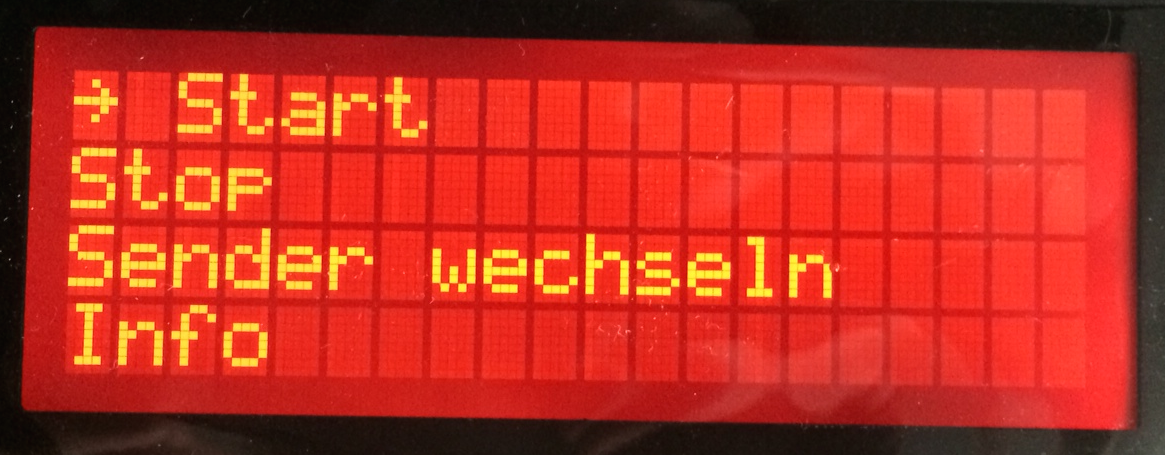
\includegraphics[width=0.7\textwidth]{Bilder/mainmenu.png}
  \caption{Hauptmenü}
  \label{fig:mainmenu}
\end{figure}

\subsubsection{Start}
Dieser Menüpunkt startet die Wiedergabe des ersten Radiosenders. Nach Auswahl dieses Menüpunktes wechselt das Programm in das Now-Playing Menü.

\subsubsection{Stop}
Dieser Menüpunkt beendet die Wiedergabe.

\subsubsection{Sender wechseln}
Dieser Menüpunkt wechselt den Radiosender. Es sind drei Radiosender fest im Programm eingetragen. Ein Druck auf den Button wechselt den Radiosender und das Programm wechselt in das Now-Playing Menü.
\subsubsection{Info}
Dieser Menüpunkt zeigt die IP-Adresse des Radios an.
\subsubsection{Beenden}
Dieser Menüpunkt beendet das Programm und fährt den Raspberry herunter, sodass er ausgeschaltet werden kann.


\subsection{Now-Playing Menü}
Das Now-Playing Menü wird angezeigt, wenn ein Radiosender läuft. Es werden der Name des Radiosenders, der Titel des aktuellen Liedes und die Uhrzeit angezeigt.
\begin{figure}[H] 
  \centering
     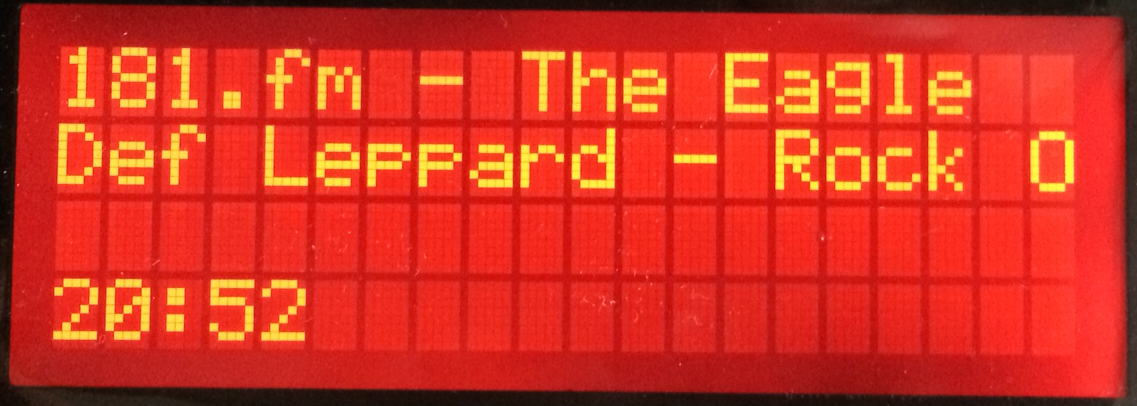
\includegraphics[width=0.7\textwidth]{Bilder/playmenu.png}
  \caption{Now-Playing Menü}
  \label{fig:playmenu}
\end{figure}